\documentclass[a4paper, 10pt]{article}
\usepackage[margin=0.5in]{geometry}
\usepackage{graphicx}
\usepackage{listings}
\usepackage{amsmath}
\usepackage{color}
 
\definecolor{dkgreen}{rgb}{0,0.6,0}
\definecolor{gray}{rgb}{0.5,0.5,0.5}
\definecolor{mauve}{rgb}{0.58,0,0.82}
 
\lstset{ %
  language=Matlab,                % the language of the code
  basicstyle=\footnotesize,           % the size of the fonts that are used for the code
  numbers=left,                   % where to put the line-numbers
  numberstyle=\tiny\color{gray},  % the style that is used for the line-numbers
  stepnumber=2,                   % the step between two line-numbers. If it's 1, each line 
                                  % will be numbered
  numbersep=5pt,                  % how far the line-numbers are from the code
  backgroundcolor=\color{white},      % choose the background color. You must add \usepackage{color}
  showspaces=false,               % show spaces adding particular underscores
  showstringspaces=false,         % underline spaces within strings
  showtabs=false,                 % show tabs within strings adding particular underscores
  frame=single,                   % adds a frame around the code
  rulecolor=\color{black},        % if not set, the frame-color may be changed on line-breaks within not-black text (e.g. commens (green here))
  tabsize=2,                      % sets default tabsize to 2 spaces
  captionpos=b,                   % sets the caption-position to bottom
  breaklines=true,                % sets automatic line breaking
  breakatwhitespace=false,        % sets if automatic breaks should only happen at whitespace
  title=\lstname,                   % show the filename of files included with \lstinputlisting;
                                  % also try caption instead of title
  keywordstyle=\color{blue},          % keyword style
  commentstyle=\color{dkgreen},       % comment style
  stringstyle=\color{mauve},         % string literal style
  escapeinside={\%*}{*)},            % if you want to add a comment within your code
  morekeywords={*,...}               % if you want to add more keywords to the set
}
\begin{document}
\title {Pattern Recognition EN2202 \\ Assignment 1}
\author{Radu-Mihai Pana-Talpeanu rmpt@kth.se \\Maria Gerontini mger@kth.se}
\maketitle

\section{Verifying the Markov Chain and HMM Sources}
\begin{align}
\nonumber
&q= \left( \begin{array}{c}
0.75 \\
0.25 \\ \end{array} \right) 
A= \left( \begin{array}{cc}
0.99 & 0.01\\
0.03 & 0.97 \\ \end{array} \right) 
B= \left( \begin{array}{c}
b_1(x)\\
b_2(x) \\ \end{array} \right)
\end{align}


\begin{align}
\nonumber &P(S_1=1)=0.75 \\
\nonumber &P(S_1=2)=0.25 \\
\nonumber &P(S_2=1)=P(S_1=1)*a_{11} + P(S_1=2)*a_{21} = 0.75*0.99 + 0.25*0.03 = 0.75 \\
\nonumber &P(S_2=2)=P(S_1=1)*a_{12} + P(S_1=2)*a_{22} = 0.75*0.01 + 0.25*0.97 = 0.25 
\end{align}

It can be seen that as time steps go by the probabilities that the model is in state 1 or 2 remain constant: 0.75 and 0.25 respectively.
By generating a sequence of 10000 states with the rand function we obtained the following results: state 1 occurred 7649 times and state 2 occurred 2351 times, thus confirming the theoretical calculations.
Let us now calculate the theoretical values of the mean and variance of the observed values:
\begin{align}
\nonumber E[X_t]&=\mu_X=\sum\limits_{i=1}^{2}P(S_t=i)*E[X_t|S_t=i]= \\
\nonumber &=P(S_t=1)*E[X_t|S_t=1]+P(S_t=2)*E[X_t|S_t=2] = \\
\nonumber &=0.75*\mu_1 + 0.25*\mu_2 = 0+0.75 = \\
\nonumber &=0.75
\end{align}
MATLAB's mean function gives us the following result: 0.7276. If we would have generated more than 10000 observations the value would move asimptotically towards the theoretical number of 0.75. 

We now proceed to calculate the variance of the observed values. The distribution f(x) that generates the numbers is given by $f(x)=0.75*N(0,1) + 0.25*N(3,4)$, that is, a Gaussian mixture with weights equal to 0.75 and 0.25 generates the sequence of scalars that, as we calculated above, has a mean of 0.75. The variance is given by: $\sigma^2=\sum\limits_{j=1}^{2}w_j(\sigma_j^2+\mu_j^2)-\mu^2 = 0.75*(1+0)+0.25*(4+9)-0.75^2=3.4375$. The experimental value after generating 10000 observations supports this result.

We then generated 500 observations from the HMM in order to view the nature of the randomness. As expected, the values fall within the calculated range and, moreover, the difference in variance of the 2 distributions can be seen by looking at how spread out around the mean each sample is. Another important aspect is that we get a hint about which state the model is in at every time step: when the values generated are around 3, we are probably in state $S_2$, as $\mu_2=3$, whereas if we get values close to 0, we are most likely in state $S_1$.
\begin{center}
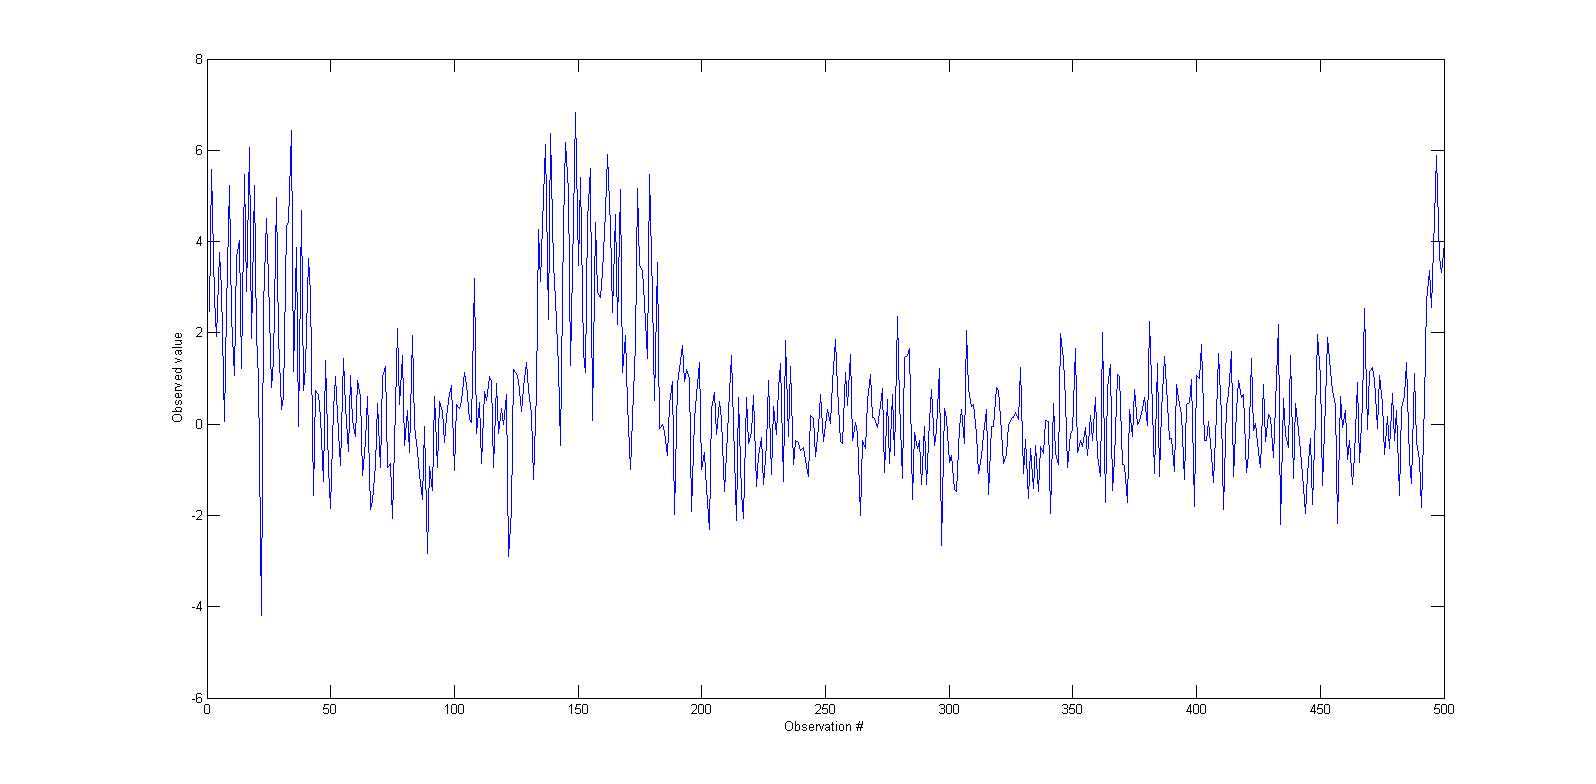
\includegraphics[scale=0.33]{500.png}
\end{center}

It comes as no surprise that when we equalize the means $\mu_1=\mu_2=0$ of the 2 distributions we can no longer ``guess'' the state transitions by looking at the plot. We get all the numbers spread around 0:
\begin{center}
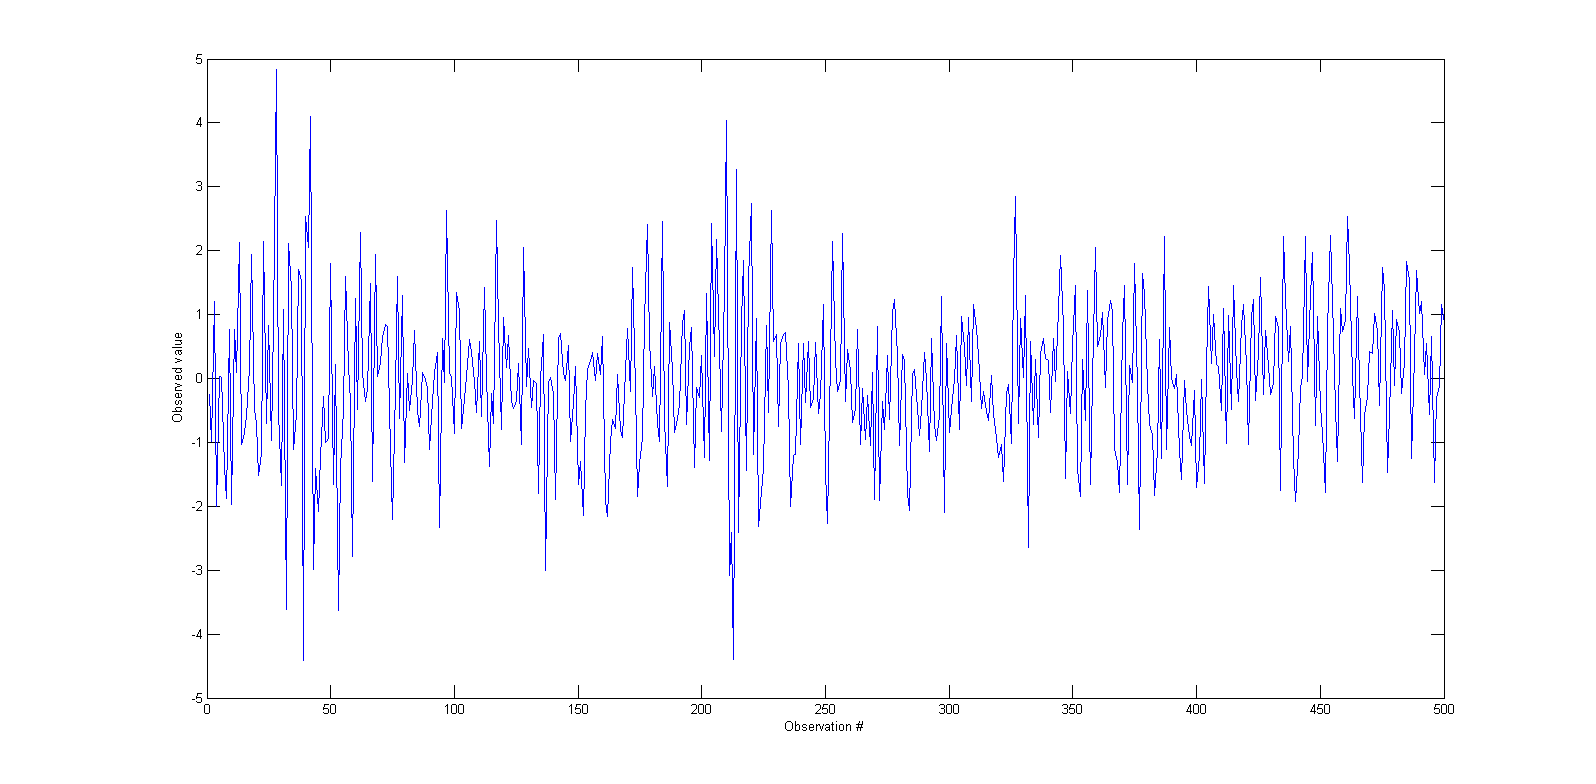
\includegraphics[scale=0.4]{500b.png}
\end{center}

Let us now test the finite duration Markov chain. We used the following values:
\begin{align}
\nonumber
&q= \left( \begin{array}{c}
0.5 \\
0.5 \\ \end{array} \right) 
A= \left( \begin{array}{ccc}
0.6 & 0.39 & 0.01\\
0.4 & 0.59 & 0.01 \\ \end{array} \right) 
B= \left( \begin{array}{c}
N(0,1)\\
N(3,4) \\ \end{array} \right)
\end{align}

After running the code to generate 500 observations from this HMM we concluded that it works as intended, since we get state sequences of length anywhere between 10 and a few hundred. If the values in the last column of the A matrix would be higher, the model would exit quite fast. But even with such a low value, the chain still ``ends'' before reaching 300 states, after running the code 10 times.

Finally, we tested to see if our code can handle vector output. We used a 2-D Gaussian distribution and generated 500 values. It successfully terminated and the resulting values were in the correct range.

\section{Code}
We present the code written for this part of the project, starting with the rand function in the @DiscreteD class:
\lstinputlisting{randDiscreteD.m}
The rand method in the @MarkovChain class:
\lstinputlisting{randMarkovChain.m}
The rand method in the @HMM class:
\lstinputlisting{randHMM.m}
Lastly, the main script:
\lstinputlisting{part1.m}
\end{document}